%% Beispiel-Präsentation mit LaTeX Beamer im KIT-Design
%% entsprechend den Gestaltungsrichtlinien vom 1. August 2020
%%
%% Siehe https://sdqweb.ipd.kit.edu/wiki/Dokumentvorlagen

%% Beispiel-Präsentation
\documentclass{sdqbeamer} 
 \usepackage{xcolor}
%% Titelbild
\titleimage{banner_2020_kit}

%% Gruppenlogo
\grouplogo{} 

%% Gruppenname
%\groupname{Institut für Informationssicherheit und Verlässlichkeit (KASTEL)}

% Beginn der Präsentation

\title[Refaktorisierung einer Architekturanalyse für Vertraulichkeit]{Refaktorisierung einer Architekturanalyse für Vertraulichkeit}
\subtitle{Praktikum Ingeneursgemäße Softwareentwicklung \hspace{5cm}Betreuer: Frederik Reiche} 
\author[Alina Valta]{Alina Valta}

\date[10.\,03.\,2022]{10. März 2022}

% Literatur 
 
\usepackage[citestyle=authoryear,bibstyle=numeric,hyperref,backend=biber]{biblatex}
\addbibresource{presentation.bib}
\bibhang1em
\begin{document}

\renewcommand{\figurename}{Abb}
%Titelseite
\KITtitleframe

%Inhaltsverzeichnis
%\begin{frame}{Inhaltsverzeichnis}
%\tableofcontents
%\end{frame}

\section{Vertraulichkeitsanalyse}

\begin{frame}{Motivation}
	\begin{columns}
	\column{.45\textwidth}
	Komponenten basierte Softwareentwicklung:
	\begin{itemize}
		\item Wiederverwendbare Komponenten
		\item Komposition von Komponenten
	\end{itemize}
	\column{.5\textwidth}
	
\includegraphics[width=0.7\textwidth]{images/CBSE_example.png}
	\end{columns}
\vspace{0.05\textheight}
	Vertraulichkeitsanalyse (\cite{kramer2017model})
	\begin{itemize}
		\item Vertrauliche Daten überschreiten Komponenten-Grenzen
		\item Probleme auf Architekturebene erkennen
	\end{itemize}
\vspace{0.05\textheight}
$\Rightarrow$ kompositorische Analyse notwendig
\end{frame}

\begin{frame}{Vertraulichkeitsanalyse}{Architekturebene}
\begin{columns}[c]
	\column{.25\textwidth}
	\centering
	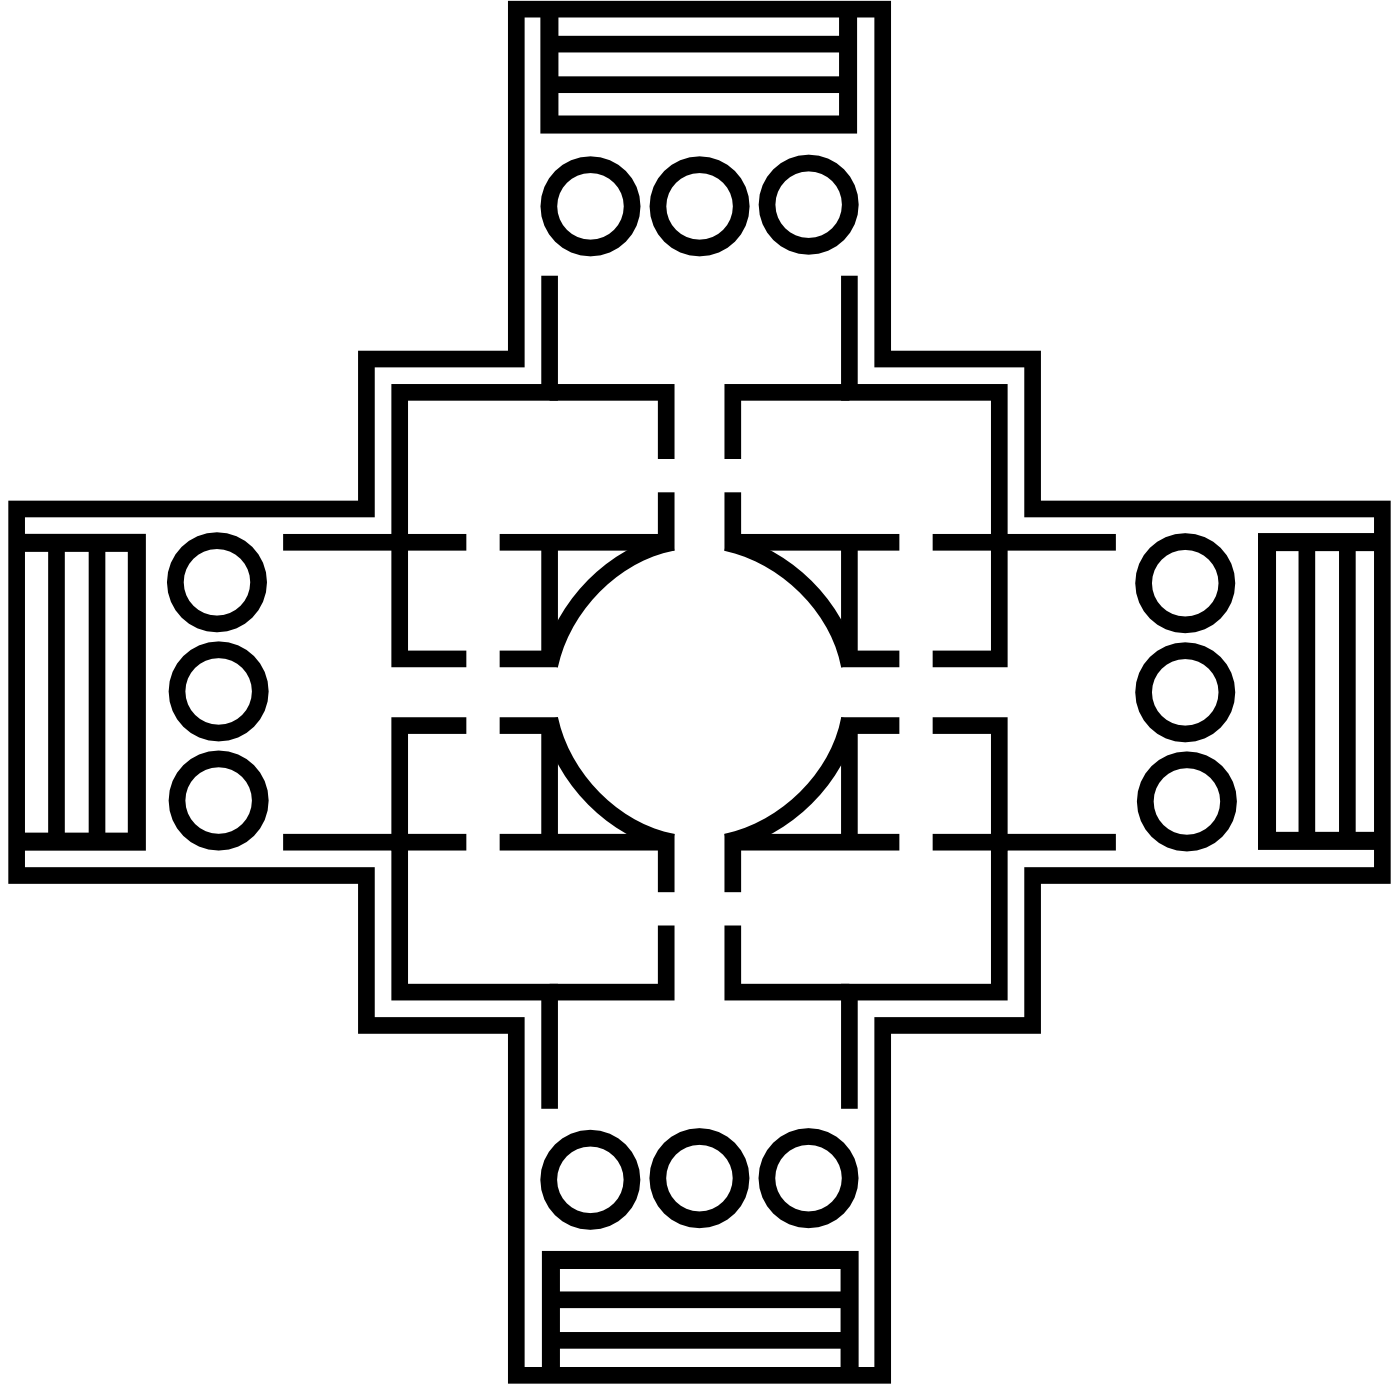
\includegraphics[width=0.6\textwidth]{images/Palladio-logo.png}
	\vspace{0.05\textheight}
	\column{.25\textwidth}
	\centering
	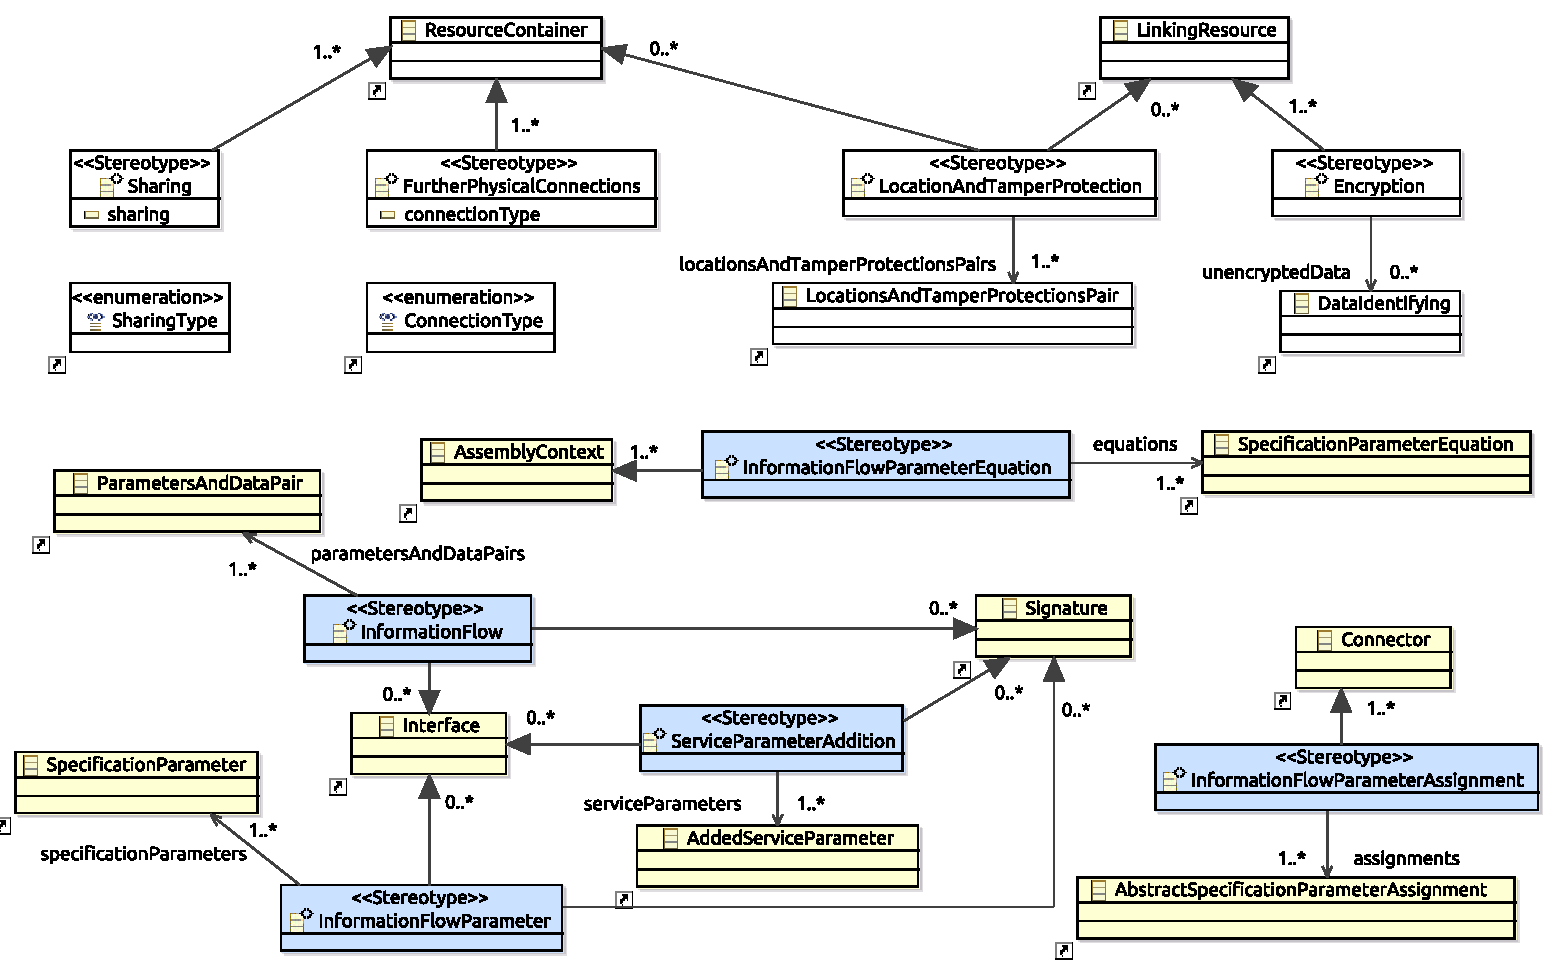
\includegraphics[width=0.9\textwidth]{images/confidentiality_profile.pdf}
	%\includegraphics[width=0.9\textwidth]{images/WordCloud.png}
	\vspace{0.05\textheight}
	\column{.25\textwidth}
	\texttt{\footnotesize dataSet(2).\\
		parametersAndDataPair(8).\\
		parameterSources(8,[return]).\\
		dataTargets(8,[5,6,7,4]).}
	\column{.25\textwidth}
	\texttt{\tiny isInSecureWithRespectTo(guest)\\
+- accessibleParameters(guest,return(getId))\\
| +- linksDataAccessibleBy(guest,wireless)\\
| | +- linkAccessibleBy(guest,wireless)\\
| | | +- linkLocation(wireless)
| | | ‘- locationsAccessibleBy(guest)}
\end{columns}
\begin{columns}\centering
	\column{.25\textwidth}
	\centering
	\textbf{Palladio Component Model}
	\vspace{0.05\textheight}
	\column{.25\textwidth}
	\centering
	\textbf{Confidentiality Model}
	\column{.25\textwidth}
	\centering
	\textbf{Prolog Prädikate}
	\column{.25\textwidth}
	\centering
	\textbf{Analyse Ergebnis}
\end{columns}
\begin{columns}\centering
\column{.1\textwidth}
\column{.25\textwidth}
\centering
$\longrightarrow$ \\
Confidentiality4CBSE\footnotemark[1]
\column{.25\textwidth}
\centering
$\longrightarrow $\\
PCM2Prolog\footnotemark[2]
\column{.25\textwidth}
\centering
$\longrightarrow$ \\
\textcolor{gray}{Haskalladio}
\column{.1\textwidth}
\end{columns}
\footnotetext[1]{https://github.com/KASTEL-SCBS/Confidentiality4CBSE}
\footnotetext[2]{https://github.com/KASTEL-SCBS/PCM2Prolog}
\end{frame}	


\begin{frame}{Vertraulichkeitsmodellierung}{Datenfluss}

	DataSet
	\begin{itemize}
		\item Menge an Ein- und Ausgabedaten von Komponenten
		\item Trennung nach Benutzergruppen, Zweck der Informationen, ...
	\end{itemize}
	\vspace{0.05\textheight}
	InformationFlow
		\begin{itemize}
			\item Ordnet Daten DataSets zu
			\item Art der Daten:
			\begin{columns}
				\column{.05\textwidth}
				\column{.25\textwidth}
				\begin{itemize}
					\item Parameter
					\item Rückgabewert
					\item Aufruf der Funktion
					\item Größe von Parametern
				\end{itemize}
				\column{.65\textwidth}
				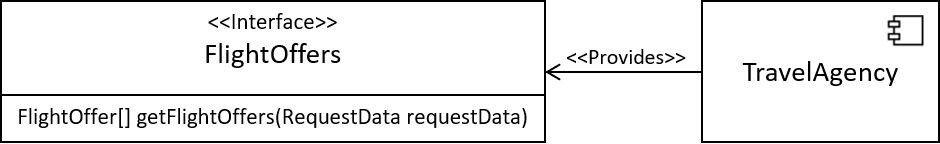
\includegraphics[width=0.9\textwidth]{images/interface.png}
				\vspace{0.05\textheight}
			\end{columns}
		\end{itemize}
\end{frame}
	
\begin{frame}{Vertraulichkeitsmodellierung}{Ressourcen}
	\begin{columns}
		\column{0.5\textwidth}
ConnectionType
	\begin{itemize}
		\item Hat ein ResourceContainer zusätzlich mögliche Verbindungen?
	\end{itemize}
\vspace{0.05\textheight}
SharingType
\begin{itemize}
	\item Laufen auf dem ResourceContainer noch andere Programme?
\end{itemize}
\vspace{0.05\textheight}
Encryption
\begin{itemize}
	\item Werden Daten unverschlüsselt übertragen?
\end{itemize}
\column{0.45\textwidth}
\end{columns}
\end{frame}	

\begin{frame}{Vertraulichkeitsmodellierung}{Maßnahmen und Angreifer}
	%\begin{columns}
		%\column{0.4\textwidth}
		Location
		\begin{itemize}
			\item Geographische Orte oder Sicherheitslevel
		\end{itemize}
		\vspace{0.05\textheight}
		TamperProtection
		\begin{itemize}
			\item Maßnahmen gegen Manipulation
		\end{itemize}
	\vspace{0.05\textheight}
	Angreifer und Benutzer des Systems
	\begin{itemize}
		\item Welche DataSets dürfen bekannt sein?
		\item Welche TamperProtections kann/will der Angreifer umgehen?
		\item Zu welchen Locations hat der Angreifer Zugriff?
	\end{itemize}
	%	\column{0.55\textwidth}
	%	\includegraphics[width=0.9\textwidth]{images/TamperProtectionImage.png}
	%\end{columns}
\end{frame}	

\section{Entfernen Profil-Mechanismus}
\begin{frame}{Bisheriges Modell}{Profil-Mechanismus}
\begin{columns}
	\column{0.55\textwidth}
Confidentiality Modell: 
\begin{itemize}
	\item Definiert Klassen zum Modellieren von DataSet, Maßnahmen, Angreifer, ...
\end{itemize}
\vspace{0.05\textheight}
Confidentiality Profil:
\begin{itemize}
	\item Verbindet PCM Elemente und Confidentiality Modell
	\item Zusammenfassung von mehreren Stereotypen
	\begin{itemize}
		\item Stereotyp erweitert eine oder mehrere PCM Klassen
		\item Stereotyp hat Referenzen zu Elementen aus dem Confidentiality Modell
	\end{itemize}
	
\end{itemize}%
$\Rightarrow$ Probleme mit Eclipse und unübersichtlich
\column{0.02\textwidth}\centering
\only<2->{\Large$\Rightarrow$}
\column{0.35\textwidth}
\only<1>{
\begin{figure}
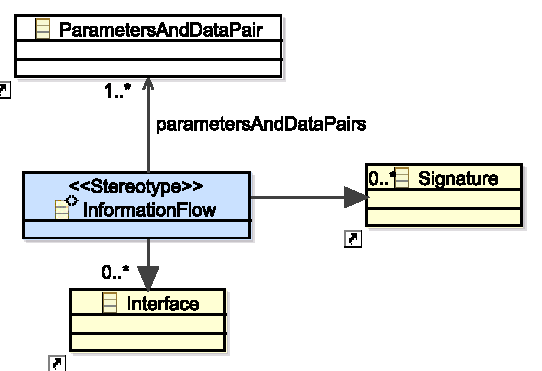
\includegraphics[width=\textwidth]{images/repsoitory_stereotype.pdf}
		\caption{Beispiel Stereotyp}
\end{figure}
}
\only<2->{
\textbf{Lösung:} Stereotypen ersetzen
\begin{itemize}
	\item Neue Modell Klassen
	\item Existierende Klassen erweitern
	\item Referenz zu PCM Elementen
\end{itemize}
}
\end{columns}
\end{frame}	
\begin{frame}{Entfernen Profil-Mechanismus}{Beispiel InformationFlow}
	\begin{columns}
		\column{0.4\textwidth}\centering
		\begin{figure}
			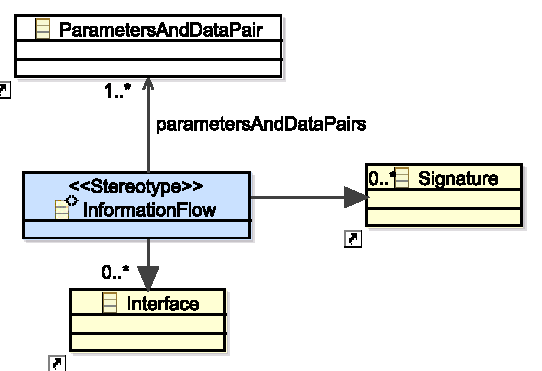
\includegraphics[width=\textwidth]{images/repsoitory_stereotype.pdf}
			\caption{InformationFlow Stereotyp kann auf Signaturen und Interfaces angewandt werden}
		\end{figure}
		\column{0.05\textwidth}\centering
		\LARGE{$\rightarrow$}
		\column{0.5\textwidth}\centering
		\begin{figure}
			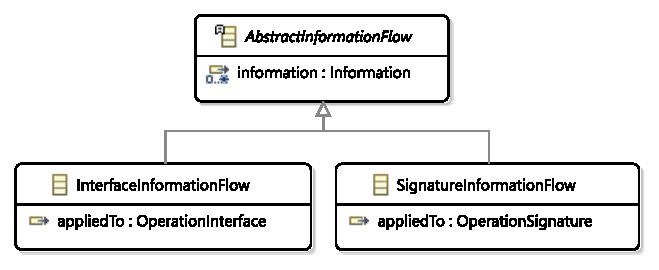
\includegraphics[width=\textwidth]{images/repository.pdf}
			\caption{Modell nach Entfernen des Stereotyps \linebreak Information Klasse ersetzt ParameterAndDataPair}
		\end{figure}
	\end{columns}
\end{frame}

\section{Information Modellierung}
\begin{frame}{Bisheriges Modell}{Information Modellierung}
		\begin{columns}
		\column{0.55\textwidth}
		Modellieren der Ein- und Ausgabedaten von Komponenten
		\begin{itemize}
			\item Zuordnung von DataSets und Daten einer Operation erfolgt über Strings
			\begin{itemize}
				\item \texttt{  ''requestData''}
				\item \texttt{  ''$\backslash$return''}
				\item \texttt{  ''$\backslash$call''}
				\item \texttt{  ''*''}
				\item \texttt{  ''sizeof(*)''}
			\end{itemize}
			\item Probleme:
			\begin{itemize}
				\item implizite Referenzen
				\item Syntax muss bekannt sein
				\item Verwechslungsgefahr bei gleichnamigen Parametern
			\end{itemize}
		\end{itemize}
		$\Rightarrow$ soll explizit modelliert werden
		\column{0.35\textwidth}
		\begin{center}
			\begin{figure}
				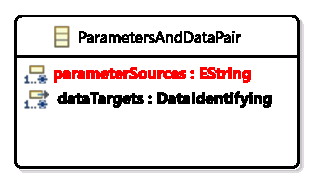
\includegraphics[width=0.7\textwidth]{images/ParameterAndDataPair.pdf}
				\caption{Zuordnung von Daten und DataSets über Strings im ursprünglichen Modell}
			\end{figure}
		\end{center}
		\vspace{0.02\textheight}
		
	\end{columns}	
\end{frame}

\begin{frame}{Informations-Modellierung}{String durch Referenz ersetzten}
	\begin{columns}
		\column{0.3\textwidth}\centering
		\begin{figure}
			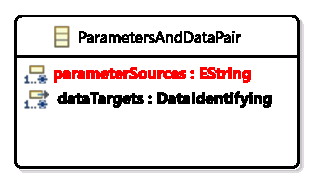
\includegraphics[width=0.9\textwidth]{images/ParameterAndDataPair.pdf}
			\caption{Zuordnung von Daten und DataSets über Strings im ursprünglichen Modell}
		\end{figure}
		\column{0.05\textwidth}\centering
		\LARGE{$\rightarrow$}
		\column{0.6\textwidth}\centering
		\begin{figure}
			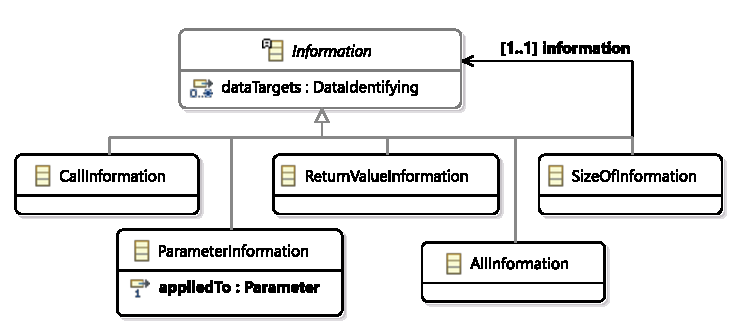
\includegraphics[width=\textwidth]{images/information.pdf}
			\caption{Modellierung der Information als eigene Klassen im neuen Modell}
		\end{figure}
	\end{columns}
\end{frame}

\section{PCM2Prolog}
\begin{frame}{PCM2Prolog}{Modellinstanz zu Prolog Code}
	\begin{itemize}
		\item Geschrieben in Xtend
		\item Reflective-API wird verwendet um Entitäten auf Prolog Prädikate abzubilden
		\item Filter bestimmt relevante Entitäten und Referenzen
	\end{itemize}
\vspace{0.05\textheight}	
	\begin{columns}
		\column{0.5\textwidth}\centering
		\begin{figure}
			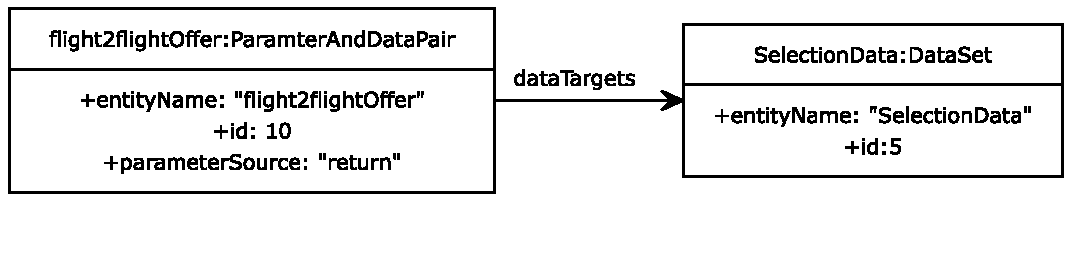
\includegraphics[width=\textwidth]{images/pcm2prologUml.pdf}
			\caption{Beispiel Modellinstanz \linebreak Filter Entitäten: ParameterAndDataPair, DataSet \linebreak Filter Referenzen: id, dataTargets}
		\end{figure}
		\column{0.05\textwidth}\centering
		\LARGE{$\rightarrow$}
		\column{0.35\textwidth}
		\begin{figure}\raggedright 
		\texttt{parametersAndDataPair(10).\\
			parameterSources(10,[return]).\\
			dataTargets(10,[5]).\\ \vspace{0.025\textheight}
			dataSet(5).}
		\caption{Prolog Prädikate für diese Modell-Instanz}
		\end{figure}
	\end{columns}
\end{frame}	
\begin{frame}{PCM2Prolog}{Anpassungen}
	Änderungen des Modells sollen sich nicht auf den Prolog Code auswirken
	\vspace{0.05\textheight}
	\begin{itemize}
		\item Dispatch-Methoden für Entitäten, die nicht automatisch generiert werden können \\ \vspace{0.025\textheight}
		\texttt{def dispatch String generateDeeplyCorrectly(EObject e) $\{$
				return super.generateDeeply(e)
		$\}$}\\
		\texttt{def dispatch String generateDeeplyCorrectly(AbstractResourceProtection rp) $\{...\}$} \\ \vspace{0.025\textheight}
		\item Richtung der ursprüngliche Stereotypen Referenzen
		\begin{itemize}
			\item \textit{vorher:} PCM $\rightarrow$ Modell (über Stereotyp) \\
			\textit{jetzt:}\hspace{0.019\textwidth} Modell $\rightarrow$ PCM
			\vspace{0.02\textheight}
			\item Map für jeden früheren Stereotyp
			\begin{itemize}
				\item Key: PCM Element, Value: Set an Ids
			\end{itemize}
			\item Beim Verarbeiten der Confidentiality Klassen wird die Map gefüllt
			\item Am Ende: erzeuge Prädikate aus den Map Elementen
		\end{itemize}
	\end{itemize}
\end{frame}
\section{Evaluierung}
\begin{frame}{Evaluierung}{Automatisch Überprüfung der Ergebnisse}
	Modellierung der Beispiel Projekte mit dem neuen Modell:
	\begin{itemize}
		\item Gleiche Ids verwenden
	\end{itemize}
\vspace{0.05\textheight}
	Automatischer Vergleich des Prolog Codes:
	\begin{itemize}
		\item Prolog Datei vorverarbeiten:
		\begin{itemize}
			\item Listen innerhalb von Prädikaten sortieren:
			\hspace{0.05\textwidth}\texttt{prädikatName(5, [''b'',''c'',''a'']).} $\Rightarrow$ \\ \hspace{0.408\textwidth} \texttt{prädikatName(5, [''a'',''b'',''c'']).}
			\item Zeilen der Datei sortieren
			\item Leerzeilen entfernen
		\end{itemize}
		\item Ausgabe mit \texttt{diff} vergleichen
	\end{itemize}
\end{frame}
\begin{frame}{Evaluierung}{Ergebnisse}
		Projekte \texttt{cloudscenario-minimized}\footnote{https://github.com/KASTEL-SCBS/Examples4SCBS/tree/master/bundles/edu.kit.kastel.scbs.cloudscenario-minimized} und \texttt{iflowexample}\footnote{https://github.com/KASTEL-SCBS/Examples4SCBS/tree/master/bundles/edu.kit.kastel.scbs.iflowexample}:
		\begin{itemize}
			\item Gleicher Prolog Code konnte generiert werden
		\end{itemize}
		\vspace{0.05\textheight}
		Grenzen der Refaktorisierung
		\begin{itemize}
			\item Kommentare
			\item Wiederverwendung von Hilfsklassen (z.B. ParameterAndDataPairs) nicht mehr möglich\\ $\rightarrow$ PrologCode ändert sich
		\end{itemize}
	$\Rightarrow$ Bis auf die Wiederverwendung von Hilfsklassen können alle Modellinstanzen in das neue Modell übertragen werden, ohne dass der Prolog Code sich ändert.
\end{frame}
\section{Fazit}
\begin{frame}{Fazit}
	\begin{columns}[t]
		\column{0.45\textwidth}
		Problem:
		\begin{itemize}
			\item Profil-Mechanismus + Eclipse
			\item String Referenzen
		\end{itemize}
		\column{0.45\textwidth}
		Idee:
			\begin{itemize}
			\item Refaktorisierung des Modells
		\end{itemize}
	\end{columns}
	\vspace{0.05\textheight}
	\begin{columns}[t]
		\column{0.45\textwidth}
		Vorgehen:
		\begin{itemize}
		\item Neue Modell Klassen statt Stereotypen
		\item Explizite Referenzen statt Strings
		\item PCM2Prolog angepasst um Prolog Code nicht zu verändern
		\end{itemize}
	\column{0.45\textwidth}
	Ergebnis:
		\begin{itemize}
		\item Erfolgreiche Refaktorisierung zweier Beispiel Projekte
		\item Gleicher Prolog Code bis auf die Wiederverwendung von Hilfsklassen
\end{itemize}
\end{columns}
	
\end{frame}

\begin{frame}{Referenzen}
	\nocite{*}
	\printbibliography
\end{frame}
\appendix
\beginbackup

 %% ----------------------------------------
%% | /Test-Folie mit definierten Farben |
%% ----------------------------------------
\backupend

\end{document}